% vim: ft=tex sts=2 sw=2 et:

\documentclass{classrep}
\usepackage[utf8]{inputenc}
\usepackage{hyperref}
\usepackage{graphicx}

\studycycle{Informatyka, studia dzienne, inż. I st.}
\coursesemester{VII}

\coursename{Technologie symulacji komputerowych}
\courseyear{2011/2012}

\courseteacher{dr Jan Rogowski}
\coursegroup{poniedziałek, 08:30}

\author{\studentinfo{Paweł Placzyński}{143072}}

\title{Symulacja wahadła złożonego}

\begin{document}
\maketitle

\section{Cel}

Celem zadania jest stworzenie aplikacji umożliwiającej przeprowadzenie symulacji
ruchu wahadła złożonego przy danym stanie początkowym.

\section{Teoria}

\subsection{Wahadło matematyczne}

\subsubsection{Definicja}

Wahadło matematyczne \cite{skorko} to~punkt materialny o masie $ m $ zawieszony
na~nierozciągliwej i~nieważkiej nici długości $ l $. Jest to~idealizacja wahadła
fizycznego.


Ważną cechą wahadła fizycznego i~matematycznego jest niezależność okresu drgań
od~maksymalnego wychylenia dla niewielkich wychyleń wahadła.

\subsubsection{Analiza ruchu}

Na~punkt materialny działa stała siła grawitacji. Gdy wahadło odchylone jest
z~położenia równowagi, składowa siły grawitacji wzdłuż nici jest równoważona
przez nić, a~składowa prostopadła do~nici działająca w~kierunku punktu równowagi
nadaje ciału przyspieszenie. Ruch ciała ograniczony nicią jest ruchem
po~okręgu. Z~definicji przyspieszenia kątowego oraz z~II zasady dynamiki dla
ruchu punktu materialnego po~okręgu, dla kątów wyrażonych w~mierze łukowej kąta,
wynikają zależności \cite{tablice}:

\begin{equation}
  \begin{array}{c}
    \varepsilon = \frac{d^{2}\theta }{dt^{2}} \\
    -mg l \sin \theta = ml^{2} \cdot \frac{d^{2}\theta }{dt^{2}}
  \end{array}
\end{equation}

Dla małych wychyleń, $ \theta $ jest bliskie zera, wówczas funkcję sinus można
przybliżyć jej argumentem, co~prowadzi do~równania:

\begin{equation}
  \frac{d^{2}\theta }{dt^{2}}+\omega ^{2}\theta = 0
\end{equation}

Powyższe równanie jest równaniem ruchu drgającego harmonicznego, którego ogólna
postać jest dana wzorem:

\begin{equation}
  \frac{d^{2}\theta }{dt^{2}}+\omega ^{2}\theta = 0
\end{equation}

gdzie $ \omega $ jest częstością kołową drgań a~$ T $ -- okresem. Wynika stąd,
że~okres drgań wynosi:

\begin{equation}
  T = 2\pi \sqrt{\frac{l}{g}}
\end{equation}

\subsection{Wahadło fizyczne}

\subsubsection{Definicja}

Wahadło fizyczne \cite{skorko} to~bryła sztywna, która może wykonywać obroty
dookoła poziomej osi przechodzącej ponad środkiem ciężkości tej bryły.

\subsubsection{Analiza ruchu}

Wzór na~okres drgań wahadła fizycznego dla małych wychyleń \cite{tablice}:

\begin{equation}
  T = 2\pi \sqrt{\frac{I}{mgd}}
\end{equation}

\subsection{Wahadło złożone}

Wahadłem złożonym nazywamy pewien łańcuch wahadeł (matematycznych, bądź
fizycznych), kolejno zawieszonych na~sobie.

\subsection{Wahadło Foucaulta}

\subsubsection{Definicja}

Dzięki działaniu siły Coriolisa spowodowanej obrotem Ziemi \cite{tablice}:

\begin{equation}
  \vec{F}_C = -2m(\vec{\omega} \times \vec{v})
\end{equation}

płaszczyzna drgań wahadła ulega powolnemu obrotowi. Ściśle mówiąc płaszczyzna
wahań jest stała w~układzie inercjalnym, zatem musi obracać się w~układzie
wirującym.


Obserwowany okres obrotu płaszczyzny ruchu wahadła można zapisać
w~postaci przybliżonej jako \cite{tablice}:

\begin{equation}
  T \approx \frac{24 \mathrm{h}}{\sin\varphi}
\end{equation}

gdzie $ \varphi $, to~szerokość geograficzna, na~której znajduje się wahadło.

\section{Realizacja zadania}

\subsection{Technologie}

Do~realizacji zadania użyto języka \texttt{python} zgodnego z~interpreterem
w~wersji 2.7.1+, modułu \texttt{pygame} udostępniającego środowisko dla gier
oraz~modułu \texttt{PyOpenGL} pozwalającego na~użycie w~aplikacjach pythona
rozwiązań znanej biblioteki \texttt{OpenGL}.


Do~stworzenia graficznego interfejsu użytkownika pozwalającego na~ustalenie
parametrów wejściowych symulacji użyto modułu \texttt{Tkinter} stanowiącego
API technologii \texttt{Tcl/Tk} dla aplikacji napisanych w~pythonie.


Logika programu testowana jest przy pomocy modułu \texttt{unittest} pozwalającego
na~przeprowadzenie testów jednostkowych.

\subsection{Repozytorium}

Kod źródłowy projektu dostępny jest pod repozytotium \texttt{git}, pod adresem
\url{https://github.com/placek/pendulum} na~gałęzi \texttt{master}.


Na gałęzi \texttt{ticgit} dostępny jest dziennik wykonanych zadań związanych
z~realizacją projektu. Dostęp do~dziennika możliwy jest przy użyciu narzędzia
\texttt{ticgit} (\url{https://github.com/schacon/ticgit/wiki/}).

\subsection{Osiągnięcia}

\begin{figure}[htb]
  \centering
  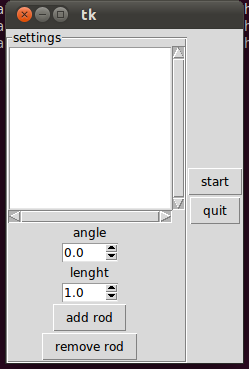
\includegraphics[scale=0.5]{img/gui.png}
  \caption{Interfejs graficzny uruchamiający/konfigurujący symulację.}
  \label{img:gui}
\end{figure}

\begin{figure}[htb]
\centering
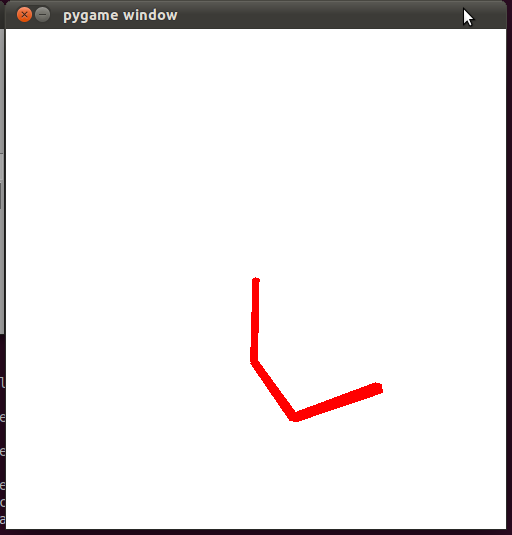
\includegraphics[scale=0.5]{img/sim.png}
\caption{Okno symulacji.}
\label{img:gui}
\end{figure}

Do~tej pory udało się:

\begin{enumerate}
  \item utworzyć środowisko graficzne pozwalające na~wyświetlenie symulowanego
  modelu (łańcucha zbudowanego z~prętów);
  \item odseparować silnik graficzny od~logiki aplikacji używając osobnego wątku;
  \item dodać GUI pozwalające na uruchomienie symulacji i~podstawową konfigurację.
\end{enumerate}


Aplikacja potrafi:

\begin{enumerate}
  \item wyświetlić okno pozwalające na~uruchomienie symulacji oraz~przeprowadzenie
  prostej konfiguracji;
  \item umożliwić tworzenie/edycję symulowanego obiektu;
  \item uruchomić okno symulacji, w~którym możliwa jest zmiana pozycji, z~której
  obserwowana jest symulacja.
\end{enumerate}


\begin{thebibliography}{0}
  \bibitem{skorko} Marta Skorko
    \textsl{Fizyka}, Warszawa 1982, PWN, wydanie VIII
  \bibitem{tablice} Witold Mizerski
    \textsl{Tablice fizyczno-astronomiczne} Warszawa 2002, Adamantan, wydanie II
\end{thebibliography}
\end{document}
